 \let\negmedspace\undefined
\let\negthickspace\undefined
\documentclass[journal]{IEEEtran}
\usepackage[a5paper, margin=10mm, onecolumn]{geometry}
%\usepackage{lmodern} % Ensure lmodern is loaded for pdflatex
\usepackage{tfrupee} % Include tfrupee package

\setlength{\headheight}{1cm} % Set the height of the header box
\setlength{\headsep}{0mm}     % Set the distance between the header box and the top of the text
\usepackage{gvv-book}
\usepackage{gvv}
\usepackage{cite}
\usepackage{amsmath,amssymb,amsfonts,amsthm}
\usepackage{algorithmic}
\usepackage{graphicx}
\usepackage{textcomp}
\usepackage{xcolor}
\usepackage{txfonts}
\usepackage{listings}
\usepackage{enumitem}
\usepackage{mathtools}
\usepackage{gensymb}
\usepackage{comment}
\usepackage[breaklinks=true]{hyperref}
\usepackage{tkz-euclide} 
\usepackage{listings}
% \usepackage{gvv}                                        
\def\inputGnumericTable{}                                 
\usepackage[latin1]{inputenc}                                
\usepackage{color}                                            
\usepackage{array}                                            
\usepackage{longtable}                                       
\usepackage{calc}                                             
\usepackage{multirow}                                         
\usepackage{hhline}                                           
\usepackage{ifthen}                                           
\usepackage{lscape}



\usepackage{amsmath,amssymb}
\usepackage{booktabs}
\usepackage{tikz}
\usetikzlibrary{arrows.meta,angles,quotes}





\begin{document}

\bibliographystyle{IEEEtran}
\vspace{3cm}

\title{4.4.19}
\author{AI25BTECH11023 - Pratik R}
% \maketitle
% \newpage
% \bigskip
{\let\newpage\relax\maketitle}

\renewcommand{\thefigure}{\theenumi}
\renewcommand{\thetable}{\theenumi}
\setlength{\intextsep}{10pt} % Space between text and floats


\numberwithin{equation}{enumi}
\numberwithin{figure}{enumi}
\renewcommand{\thetable}{\theenumi}


\section*{\textbf{Question}}
\textbf{Assertion (A):} Point P(0,2) is point of intersection of Y-axis with the line
$3x + 2y = 4$.

\textbf{Reason (R):} The distance of point $P(0,2)$ from X-axis is 2 units. 
\section*{\textbf{Solution}}
\subsection*{\textbf{The given equation can be expressed as}}
\begin{align}
    \myvec{3 & 2}x =4
\end{align}
where $n^\top = \myvec{3&2}$ and $c = 4$.

\subsection*{\textbf{Putting $P(0,2)$ in the equation of line}}
\begin{align}
n^\top P =4=c
\end{align}
Since $(0,2)$ lies on y-axis, Assertion is correct.

\subsection*{\textbf{Distance of $(x,y)$ from x-axis is $|y|$}}

Hence Reason is also correct but it is not a valid reason for assertion.
\newpage

\begin{figure}[H]
\centering
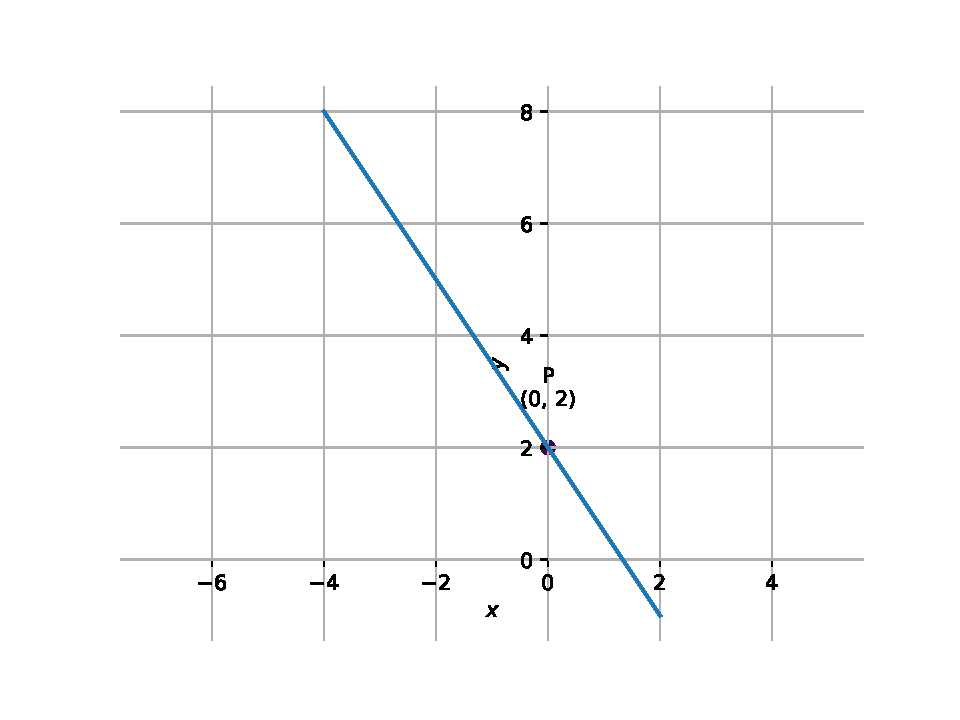
\includegraphics[width=0.7\columnwidth]{figs/fig.pdf} 
\caption{Plot of line $3x+2y=4$}
\label{}
\end{figure}
\end{document}
